
\scsubsection{Описание языка графического представления знаний интеллектуальных компьютерных систем}
\label{intro_scg}

\begin{SCn}

\scnsectionheader{\currentname}

\scnstartsubstruct

\scnidtf{Описание SCg-кода}
\scnreltovector{конкатенация сегментов}{Основные положения языка графического представления знаний ostis-систем;Описание Ядра SCg-кода;Описание Первого расширения Ядра SCg-кода;Описание Второго расширения Ядра SCg-кода;Описание Третьего расширения Ядра SCg-кода;Описание Четвертого расширения Ядра SCg-кода;Описание Пятого расширения Ядра SCg-кода;Описание Шестого расширения Ядра SCg-кода;Описание Седьмого расширения Ядра SCg-кода;Итоговый сегмент Описания Языка графического представления знаний ostis-систем}

\scnsegmentheader{Основные положения языка графического представления знаний ostis-систем}

\scnstartsubstruct

\scnheader{SCg-код}
\scnidtf{Semantic Code graphical}
\scnidtf{Язык визуального (графического) представления баз знаний ostis-систем}
\scniselement{графовый язык}
\scnexplanation{\textit{SCg-код} представляет собой способ визуализации \textit{sc-текстов} (информационных конструкций SC-кода) в виде рисунков этих абстрактных конструкций. Подчеркнем, что абстрактная \textit{графовая структура} и её рисунок (графическое изображение) -- это не одно и то же даже если они \textit{изоморфны} друг другу. \textit{SCg-код} рассматривается нами как объединение \textit{Ядра SCg-кода}, обеспечивающего изоморфное графическое изображение любого \textit{sc-текста}, а также нескольких направлений расширения этого ядра, обеспечивающих повышение компактности и "читабельности"{} текстов \textit{SCg-кода} (\textit{sc.g-текстов}).}
\scnnote{\textit{SC-код} -- это рассмотрение множества всевозможных графически представленных (визуализированных) графовых структур как \underline{универсального} языка представления знаний с соответствующим синтаксисом и семантикой.}
\scnendstruct

\scnsegmentheader{Описание Ядра SCg-кода}

\scnstartsubstruct
\scnheader{Алфавит Ядра SCg-кода}
\scnidtf{Алфавит sc.g-элементов, графически изображающих sc-элементы}
\scnrelto{ключевой знак}{Таблица. Алфавит Ядра SCg-кода}
\scnexplanation{\textit{Алфавит Ядра SCg-кода} взаимно однозначно соответствует \textit{Алфавиту SC-кода}. Указанное соответствие представлено в файле ``Таблица. Алфавит Ядра SCg-кода''.}

\scnheader{Таблица. Алфавит Ядра SCg-кода}
\scneqtable{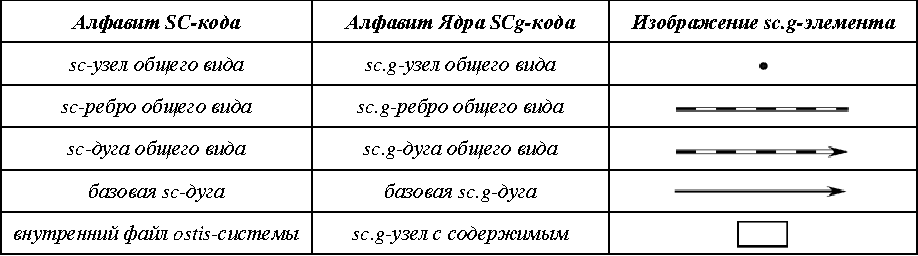
\includegraphics{figures/intro/scg/SCg-core-alphabet.pdf}}

%TODO сверить пропорции sc.g-элементов и изменить описание
\scnheader{sc.g-узел общего вида}
\scnidtf{\textit{sc.g-элемент}, являющийся графическим изображением \textit{sc-узла общего вида}}
\scnexplanation{Все \textit{sc-узлы}, не являющиеся знаками файлов, в тексте (конструкции) \textit{Ядра SCg-кода}, изображаются в виде небольших чёрных кругов одинакового диаметра, который обозначим через $\bm{d}$, и точная величина которого зависит от масштаба отображения \textit{sc.g-текста}.}

\scnheader{sc.g-ребро общего вида}
\scnidtf{\textit{sc.g-элемент}, являющийся графическим изображением \textit{sc-ребра общего вида}}
\scnexplanation{Каждое \textit{sc-ребро} в \textit{Ядре SCg-кода} изображается в виде широкой линии, в которой чередуются фрагменты со сплошной заливкой и без заливки, не имеющей самопересечений и имеющей общую толщину, равную примерно $\bm{0.7d}$.}

\scnheader{sc.g-дуга общего вида}
\scnidtf{\textit{sc.g-элемент}, являющийся графическим изображением \textit{sc-дуги общего вида}}
\scnexplanation{Каждая \textit{sc-дуга} в \textit{Ядре SCg-кода} изображается в виде широкой линии, в которой чередуются фрагменты со сплошной заливкой и без заливки, не имеющей самопересечений, имеющей общую толщину, равную примерно $\bm{0.7d}$ и имеющей изображение стрелочки на одном из концов этой линии.}

\scnheader{базовая sc.g-дуга}
\scnidtf{\textit{sc.g-элемент}, являющийся графическим изображением \textit{базовой sc-дуги}}
\scnexplanation{Каждая входящая в состав sc-текста \textit{базовая sc-дуга} в \textit{Ядре SCg-кода} изображается в виде линии произвольной формы, не имеющий самопересечений, имеющий толщину $\bm{0.4d}$, и имеющей изображение стрелочки на одном из ее концов.}

\scnheader{внутренний файл ostis-системы}
\scnidtf{sc-узел с содержимым}
\scnaddlevel{1}
\scniselement{часто используемый sc-идентификатор}
\scnaddlevel{-1}
\scnidtf{sc-узел, являющийся знаком внутреннего файла ostis-системы}
\scnidtf{sc-знак внутреннего файла ostis-системы}

\scnheader{sc.g-узел с содержимым}
\scnidtf{sc.g-узел, имеющий содержимое}
\scnidtf{sc.g-узел, являющийся знаком внутреннего файла ostis-системы}
\scnidtf{sc.g-знак внутреннего файла ostis-системы}
\scnidtf{sc.g-рамка, ограничивающая изображение (представление) внутреннего файла ostis-системы, обозначаемого этой sc.g-рамкой}
\scnidtf{sc.g-рамка}
\scnaddlevel{1}
\scnnote{\textit{sc.g-рамка} -- это всегда прямоугольник, максимальный размер которого не ограничивается, но минимальный фиксируется и соответствует \textit{sc.g-рамке}, внутри которой обозначаемый ею \textit{файл} не отображается.}
\scnaddlevel{-1}
\scnexplanation{Каждый входящий в sc-текст \textit{sc-узел, имеющий содержимое}, в \textit{Ядре SCg-кода} изображается в виде прямоугольника произвольного размера с толщиной линии $\bm{0.6d}$. Внутри этого прямоугольника отображается \textit{файл}, обозначаемый изображаемым \textit{sc-узлом}. Если нет необходимости изображать в тексте сам \textit{файл}, то \textit{sc-узел}, обозначающий такой \textit{файл}, в \textit{sc.g-тексте} изображается в виде прямоугольника со сторонами $\bm{2d}$ по вертикали и $\bm{4d}$ по горизонтали.}

\scnheader{Алфавит Ядра SCg-кода}
\scnnote{Трудно сразу поверить, что на основе такого простого алфавита можно построить удобный и \uline{универсальный} графовый язык. В рамках \textit{Документации Технологии OSTIS} мы постараемся Вас в этом убедить. Кроме того, нас не должна настораживать простота алфавита, поскольку человечество имеет большой опыт кодирования, хранения в памяти и передачи по каналам связи самых различных информационных ресурсов, используя алфавит, состоящий только из двух классов элементов -- единиц и нулей. 

Мы ведем речь о принципиально ином (графовом) способе кодирования информации в \textit{компьютерных системах}, но стараемся при этом свести это кодирование к достаточно простому алфавиту хотя бы для того, чтобы искусственно не усложнять проблему создания нового поколения компьютеров, основанных на указанном способе кодирования информации. 

Расширения \textit{Ядра SCg-кода} рассмотрим как направления перехода от текстов \textit{Ядра SCg-кода} к более компактным текстам. Но, поскольку это приводит к усложнению \textit{Синтаксиса SCg-кода} и, в первую очередь, к расширению \textit{Алфавита SCg-кода}, делать такие расширения необходимо обоснованно с учетом частоты встречаемости в рамках \textit{баз знаний ostis-систем} соответствующих фрагментов.}

\scnendstruct \scninlinesourcecommentpar{Завершили сегмент ``Описание Ядра SCg-кода''}

\scnsegmentheader{Описание Первого направления расширения Ядра SCg-кода}
\scnstartsubstruct

\bigskip
\scnheader{Первое направление расширения Ядра SCg-кода}

\scnexplanation{\textit{Первое направление синтаксического расширения Ядра SCg-кода} -- это \uline{приписывание} некоторым sc.g-элементам \textit{основных sc-идентификаторов*} (чаще всего - строковых идентификаторов, то есть имен) \textit{sc-элементов} , изображаемых этими \textit{sc.g-элементами}. Указываемые идентификаторы являются уникальным для каждого идентифицируемого (именуемого) \textit{sc.g-элемента}. Приписывание \textit{sc.g-элементам} уникальных идентификаторов дает возможность в рамках одного \textit{sc.g-текста} дублировать (копировать) некоторые \textit{sc.g-узлы} при условии, если \uline{всем} таким копиям будут приписаны соответствующие идентификаторы. Такое дублирование \textit{sc.g-узлов} является дополнительным средствам \uline{наглядного} размещения \textit{sc.g-текстов}. Кроме того, приписывание \textit{sc.g-элементу} соответствующего ему основного (уникального) \textit{sc-идентификатора*} представляет собой более компактный вариант изображения \textit{sc.g-текстов}.}

\scnheader{Пример sc.g-текста, трансформируемого по Первому направлению расширения Ядра SCg-кода}
\scneqscg{figures/intro/scg/scg_transf1.png}
\scniselement{sc.g-текст}
\scnexplanation{Здесь (в левом нижнем углу приведенного sc.g-текста) представлен \textit{sc.g-узел общего вида}, изображающий \textit{sc-узел общего вида}, которому соответствует \textit{основной sc-идентификатор*} в виде строки ``\textbf{\textit{ei}}''}
\scnrelfrom{трансформация sc.g-текста по Первому направлению расширения Ядра SCg-кода}{\scnfilescg{figures/intro/scg/scg_transf2.png}}
\scnaddlevel{1}
    \scniselement{sc.g-текст}
    \scnexplanation{\textit{sc.g-узлу общего вида} изображающему \textit{sc-узел}, внешним идентификатором которого является строка ``\textit{основной sc-идентификатор*}'' и который, соответственно является знаком \textit{бинарного ориентированного отношения}, каждая \textit{пара} которого связывает идентифицируемый \textit{sc-элемент} с его основным внешним sc-идентификатором, приписывается указанный внешний идентификатор изображаемого им \textit{sc-элемента}.}
    \scnrelfrom{трансформация sc.g-текста по Первому направлению расширения Ядра SCg-кода}{\scnfilescg{figures/intro/scg/scg_transf3.png}}
    \scnaddlevel{1}
        \scniselement{sc.g-текст} 
        \scnexplanation{В результате данной трансформации исходный \textit{sc.g-текст} трансформируется в один \textit{sc.g-общего вида}, которому приписывается \textit{основной sc-идентификатор} ``\textit{\textbf{ei}}''.}
    \scnaddlevel{-1}
\scnaddlevel{-1}


\scnheader{трансформация sc.g-текста по Первому направлению расширения Ядра SCg-кода*}
\scnidtf{Бинарное ориентированное отношение, каждая пара которого связывает исходный вид трансформируемого sc.g-текста и результат этой трансформации}
\scnnote{Подчеркнем, что рассматриваемая трансформация преобразует исходный текст Ядра \textit{SCg-кода} в текст, семантически эквивалентный, но принадлежащий не Ядру \textit{SCg-кода}, а его расширению.
}

\scnheader{синтаксическая трансформация*}
\scnidtf{синтаксическая трансформация информационной конструкции*}
\scnsuperset{синтаксическая трансформация sc.g-текста*}
\scnaddlevel{1}
\scnsuperset{трансформация sc.g-текста по Первому направлению расширения Ядра SCg-кода*}
\scnaddlevel{-1}

\scnendstruct \scninlinesourcecommentpar{Завершили сегмент "Описание первого направления расширения Ядра SCg-кода}
\bigskip

\scnsegmentheader{Описание Второго направления расширения Ядра SCg-кода}
\scnstartsubstruct

\scnheader{Второе направление расширения Ядра SCg-кода}
\scnexplanation{\textit{Второе направление расширения Ядра SCg-кода} -- это уточнение типологии \textit{константных постоянных сущностей} и расширение \textit{Алфавита Ядра SCg-кода}, позволяющее типологию \textit{константных постоянных сущностей} привести в соответствие с синтаксической типологией новых вводимых элементов \textit{Алфавита SCg-кода}. Рассмотрим подробнее sc.g-элементы, знаки \textit{константных постоянных сущностей} различного вида. Графическим признаком \textit{константных постоянных sc-узлов} в конструкциях SCg-кода является их изображение в виде \uline{окружностей} диаметра $3d$, где $d$ -- диаметр sc.g-узла общего вида. Такое изображение является более компактной записью факта принадлежности заданного sc-узла (назовем его $\bm{vi}$) классу sc-констант и классу обозначений постоянных сущностей. Запись этого факта в \textit{Ядре SCg-кода} потребует (1) явного изображения sc-узла, обозначающего класс всевозможных константных sc-элементов (класс \textit{sc-констант}), (2) явного изображения базовой sc-дуги, соединяющего изображение sc-узла, обозначающего класс sc-констант, с изображением заданного константного sc-узла, (3) явного изображение sc-узла, обозначающего класс всевозможных sc-элементов, обозначающих \textit{постоянные сущности}, (4) явного изображения базовой sc-дуги, соединяющего изображение sc-узла, обозначающего класс обозначений \textit{постоянных сущностей} с изображением рассматриваемого sc-узла $\bm{vi}$ (Смотрите \textit{Файл. Изображение спецификации sc.g-элемента средствами Ядра SCg-кода и Первого расширения Ядра SCg-кода}).

Общепринятая запись данного факта выглядит следующим образом:

``\textit{sc-константа} $\ni \bm{vi}$; \textit{постоянная сущность} $\ni \bm{v_i};$''

\textit{Константные постоянные sc-ребра} в конструкциях SCg-кода изображаются в виде двойной линии, каждая из которых имеет толщину примерно $d/7$, а расстояние между ними равно примерно $3d/7$. 

\textit{Константные постоянные sc-дуги} изображаются в виде такой же двойной линии, но со стрелочкой. Все \textit{базовые sc-дуги}, а также все sc-узлы, имеющие содержимое, по определению являются \textit{константными постоянными sc-элементами}. 

\textit{Константные sc.g-узлы}, изображаемые окружностями диаметра $3d$ и толщиной границы $d/5$, обозначают \textit{константные постоянные сущности}, о которых мало что известно, но известно то, что они не являются парами (то есть множествами, \textit{мощность*} которых равна 2) и, следовательно, не могут быть изображёны в виде sc.g-дуг или sc.g-рёбер. Но, если при этом об обозначаемой \textit{константной постоянной сущности} ($\bm{vi}$) известно, что она является классом сущностей, то явное указание принадлежности sc-элемента \textit{vi} всевозможных классов можно заменить на специальное графическое изображение sc-элемента \textit{vi}, предполагаемое указанную принадлежность. Это приводит к расширению  \textit{Алфавита SCg-кода} (см. \textit{Примеры sc.g-текстов, трансформируемых по Второму направлению расширения Ядра SCg-код}).

Аналогичным образом (см. \textit{Примеры sc.g-текстов, трансформируемых по Второму направлению расширения Ядра SCg-код}) вводятся: 
\begin{scnitemize}
\item sc.g-узел, являющийся изображением \textit{класса};  
\item sc.g-узел, являющийся изображением \textit{класса классов};  
\item sc.g-узел, являющийся изображением \textit{отношения}; 
\item sc.g-узел, являющийся изображением \textit{ролевого отношения}; 
\item sc.g-узел, являющийся изображением \textit{sc-структуры};  
\item sc.g-узел, являющийся изображением \textit{небинарной sc-связки};
\item sc.g-узел, являющийся изображением \textit{первичной сущности} (терминальной сущности, которая не является множеством, а также файлом, хранимым в памяти ostis-системы).
\end{scnitemize}

Важное место среди константных постоянных сущностей занимают \textit{константные постоянные пары принадлежности}, обозначаемое соответствующими \textit{sc.g-дугами}. Такие пары принадлежности и обозначающие их sc.g-дуги бывают позитивными, негативными и нечеткими. Константная постоянная позитивная sc.g-дуга принадлежности есть ничто иное, как \textit{базовая sc.g-дуга}. Константная постоянная негативная sc.g-дуга принадлежности изображается в виде \textit{базовой sc.g-дуги}, перечеркнутой штриховыми черточками. Константная постоянная нечёткая sc.g-дуга принадлежности изображается в виде "недочеркнутой"{} \textit{базовой sc.g-дуги}, с каждой стороны которой отображаются штрихи, по длине равные половине от длины штрихов, которыми перечеркнута \textit{константная постоянная негативная sc.g-дуга}.}

\scnheader{Файл. Изображение спецификации sc.g-элемента средствами Ядра SCg-кода и Второго направления расширения Ядра SCg-кода}
\scneqscg{figures/intro/scg/scg2ex.png}

\scnheader{Примеры sc.g-текстов, трансформируемых по Второму направлению расширения Ядра SCg-кода}
\scnstructinclusion

\scnmakeset{\scgfileitem{figures/intro/scg/scg2_ex1.png}\\
\scnaddlevel{1}
    \scnrelfrom{синтаксическая трансформация}{\scnfilescg{figures/intro/scg/scg2_ex1_1.png}}
    \scnaddlevel{1}
        \scnexplanation{Здесь вводится новый синтаксический вид \textit{sc.g-элементов} -- \textit{константный постоянный sc.g-узел общего вида}, изображаемый окружностью диаметра $3d$ и толщиной границы $d/5$.}
    \scnaddlevel{-1}
\scnaddlevel{-1};
\scgfileitem{figures/intro/scg/nodes/const_perm/sc.g_const_perm_class1.png}\\
\scnaddlevel{1}
    \scnrelfrom{синтаксическая трансформация}{\scnfilescg{figures/intro/scg/nodes/const_perm/sc.g_const_perm_class2.png}}
    \scnaddlevel{1}
        \scnexplanation{Здесь вводится новый синтаксический вид \textit{sc.g-элементов} -- \textit{константный постоянный sc.g-узел, обозначающий класс}, изображаемый как \textit{константный постоянный sc.g-узел} с "решеткой"{} внутри.}
    \scnaddlevel{-1}
\scnaddlevel{-1};
\scgfileitem{figures/intro/scg/nodes/const_perm/sc.g_const_perm_class_of_classes1.png}\\
\scnaddlevel{1}
    \scnrelfrom{синтаксическая трансформация}{\scnfilescg{figures/intro/scg/nodes/const_perm/sc.g_const_perm_class_of_classes2.png}}
    \scnaddlevel{1}
        \scnexplanation{Здесь вводится новый синтаксический вид \textit{sc.g-элементов} -- \textit{константный постоянный sc.g-узел, обозначающий класс классов}, изображаемый как \textit{константный постоянный sc.g-узел} с направленным вверх углом внутри.}
    \scnaddlevel{-1}
\scnaddlevel{-1};
\scgfileitem{figures/intro/scg/nodes/const_perm/sc.g_const_perm_norole1.png}\\
\scnaddlevel{1}
    \scnrelfrom{синтаксическая трансформация}{\scnfilescg{figures/intro/scg/nodes/const_perm/sc.g_const_perm_norole2.png}}
    \scnaddlevel{1}
        \scnexplanation{Здесь вводится новый синтаксический вид \textit{sc.g-элементов} -- \textit{константный постоянный sc.g-узел, обозначающий неролевое отношение}, изображаемый как \textit{константный постоянный sc.g-узел} с "крестиком"{} внутри.}
    \scnaddlevel{-1}
\scnaddlevel{-1};
\scgfileitem{figures/intro/scg/nodes/const_perm/sc.g_const_perm_role1.png}\\
\scnaddlevel{1}
    \scnrelfrom{синтаксическая трансформация}{\scnfilescg{figures/intro/scg/nodes/const_perm/sc.g_const_perm_role2.png}}
    \scnaddlevel{1}
        \scnexplanation{Здесь вводится новый синтаксический вид \textit{sc.g-элементов} -- \textit{константный постоянный sc.g-узел, обозначающий ролевое отношение}, изображаемый как \textit{константный постоянный sc.g-узел} с "плюсом"{} внутри.}
    \scnaddlevel{-1}
\scnaddlevel{-1};
\scgfileitem{figures/intro/scg/nodes/const_perm/sc.g_const_perm_structure1.png}\\
\scnaddlevel{1}
    \scnrelfrom{синтаксическая трансформация}{\scnfilescg{figures/intro/scg/nodes/const_perm/sc.g_const_perm_structure2.png}}
    \scnaddlevel{1}
        \scnexplanation{Здесь вводится новый синтаксический вид \textit{sc.g-элементов} -- \textit{константный постоянный sc.g-узел, обозначающий sc-структуру}, изображаемый как \textit{константный постоянный sc.g-узел} с точкой внутри.}
    \scnaddlevel{-1}
\scnaddlevel{-1};
\scgfileitem{figures/intro/scg/nodes/const_perm/sc.g_const_perm_primary_entity1.png}\\
\scnaddlevel{1}
    \scnrelfrom{синтаксическая трансформация}{\scnfilescg{figures/intro/scg/nodes/const_perm/sc.g_const_perm_primary_entity2.png}}
    \scnaddlevel{1}
        \scnexplanation{Здесь вводится новый синтаксический вид \textit{sc.g-элементов} -- \textit{константный постоянный sc.g-узел, обозначающий первичную сущность}, изображаемый как \textit{константный постоянный sc.g-узел} с  косой штриховкой внутри.}
    \scnaddlevel{-1}
\scnaddlevel{-1};
\scgfileitem{figures/intro/scg/nodes/const_perm/sc.g_const_perm_tuple1.png}\\
\scnaddlevel{1}
    \scnrelfrom{синтаксическая трансформация}{\scnfilescg{figures/intro/scg/nodes/const_perm/sc.g_const_perm_tuple2.png}}
    \scnaddlevel{1}
        \scnexplanation{Здесь вводится новый синтаксический вид \textit{sc.g-элементов} -- \textit{константный постоянный sc.g-узел, обозначающий небинарную sc-связку}, изображаемый как \textit{константный постоянный sc.g-узел} с горизонтальной линией внутри.}
    \scnaddlevel{-1}
\scnaddlevel{-1};
\scgfileitem{figures/intro/scg/arcs/const/scg_const_perm_noorien1.png}\\
\scnaddlevel{1}
    \scnrelfrom{синтаксическая трансформация}{\scnfilescg{figures/intro/scg/arcs/const/scg_const_perm_noorien2.png}}
    \scnaddlevel{1}
        \scnexplanation{Здесь вводится новый синтаксический вид \textit{sc.g-элементов} -- \textit{константное постоянное sc.g-ребро}, изображаемое двумя непрерывными параллельными линиями.}
    \scnaddlevel{-1}
\scnaddlevel{-1};
\scgfileitem{figures/intro/scg/arcs/const/scg_const_perm_orient1.png}\\
\scnaddlevel{1}
    \scnrelfrom{синтаксическая трансформация}{\scnfilescg{figures/intro/scg/arcs/const/scg_const_perm_orient2.png}}
    \scnaddlevel{1}
        \scnexplanation{Здесь вводится новый синтаксический вид \textit{sc.g-элементов} -- \textit{константная постоянная sc.g-дуга}, изображаемая двумя непрерывными параллельными линиями с общей стрелкой на одном из концов.}
    \scnaddlevel{-1}
\scnaddlevel{-1};
\scgfileitem{figures/intro/scg/arcs/const/scg_const_perm_positive1.png}\\
\scnaddlevel{1}
    \scnrelfrom{синтаксическая трансформация}{\scnfilescg{figures/intro/scg/arcs/const/scg_const_perm_positive2.png}}
    \scnaddlevel{1}
        \scnexplanation{\textit{Константная постоянная позитивная sc.g-дуга принадлежности} есть ничто иное, как \textit{базовая sc.g-дуга}.}
    \scnaddlevel{-1}
\scnaddlevel{-1};
\scgfileitem{figures/intro/scg/arcs/const/scg_const_perm_negative1.png}\\
\scnaddlevel{1}
    \scnrelfrom{синтаксическая трансформация}{\scnfilescg{figures/intro/scg/arcs/const/scg_const_perm_negative2.png}}
    \scnaddlevel{1}
        \scnexplanation{Здесь вводится новый синтаксический вид \textit{sc.g-элементов} -- \textit{константная постоянная негативная sc.g-дуга принадлежности}, изображается в виде \textit{базовой sc.g-дуги}, перечеркнутой штриховыми черточками.}
    \scnaddlevel{-1}
\scnaddlevel{-1};
\scgfileitem{figures/intro/scg/arcs/const/scg_const_perm_fuzzy1.png}\\
\scnaddlevel{1}
    \scnrelfrom{синтаксическая трансформация}{\scnfilescg{figures/intro/scg/arcs/const/scg_const_perm_fuzzy2.png}}
    \scnaddlevel{1}
        \scnexplanation{Здесь вводится новый синтаксический вид \textit{sc.g-элементов} -- \textit{константная постоянная нечеткая sc.g-дуга принадлежности}, которая изображается в виде "недочеркнутой"{} \textit{базовой sc.g-дуги}, с каждой стороны которой отображаются штрихи, по длине равные половине от длины штрихов, которыми перечеркнута \textit{константная постоянная негативная sc.g-дуга}.}
    \scnaddlevel{-1}
\scnaddlevel{-1}
}

\scnheader{Примеры sc.g-текста, записанного средствами Второго направления расширения Ядра SCg-кода}
\scnstructinclusion

\scnmakeset{\scgfileitem{figures/intro/scg/examples/scg_example_triangle.png}
\scnaddlevel{1}
\scniselementrole{пример}{sc.g-текст}
\scnexplanation{Данный sc.g-текст содержит следующую информацию:
\begin{scnitemize}
\item Сущности \textit{Треугольник ABC}~~ и ~~\textit{Треугольник CDE} являются треугольниками (принадлежат классу \textit{треугольников}). При этом известно, что площадь \textit{Треугольника CDE} в 4 раза больше, чем площадь \textit{Треугольника ABC}, но конкретные значения ллощадей не известны\char59
\item Сущность \textit{Отрезок DE} является отрезком (принадлежит классу \textit{отрезков}) и является стороной \textit{Треугольника CDE}. Кроме того, у \textit{Отрезка DE} есть длина, измерение которой в сантиметрах составляет 5. Обратите внимание, что в данном случае для упрощения понимания использовано бинарное отношение \textit{длина*}, которое является \textit{неосновным понятием} и в базе знаний заменяется на \textit{базовую sc-дугу}, связывающую величину как класс эквивалентности с конкретной сущностью, входящей в данный класс, в данном случае -- \textit{Отрезок DE}\char59  
\item Сущность \textit{Треугольник AEB} является треугольником и имеет \textit{внутренний угол*}~~~ \textit{Угол AEB}. В свою очередь, \textit{Угол AEB} является \textit{углом} и имеет \textit{косинус*}, равный 0,5\char59
\item \textit{Треугольник AEB} имеет \textit{сторону*} (не указывается, какая именно из сторон имеется в виду), \textit{средней точкой*} которой является \textit{Точка O}. В свою очередь, \textit{Точка O} является центром некоторой \textit{Окружности O}, которая относится к классу \textit{окружностей}.
\end{scnitemize}
}\scnaddlevel{-1};
\scgfileitem{figures/intro/scg/examples/scg_example_alice.png}
\scnaddlevel{1}
	\scnnote{Данный sc.g-текст основан на популярном примере, наглядно иллюстрируещем понятие семантической сети, известном как ``Социальная сеть Алисы''. Как видно из примера, данный текст описывает различные взаимосвязи персоны по имени Алиса, при этом некоторые из используемых отношений является ориентированными (например, ``работник*''), а некоторые -- неориентированными (например, ``друг*'').}
\scnaddlevel{-1}
}

\scnendstruct

\scnsegmentheader{Описание Третьего направления расширения Ядра SCg-кода}

\scnstartsubstruct

\bigskip
\scnfilelong{\textit{Третье направление расширения Ядра SCg-кода} -- это расширение его алфавита путем введения дополнительных sc.g-элементов, обозначающих \textit{константные временные сущности} различного вида. Признаком sc.g-элементов, обозначающих \textit{константные временные сущности} являются точечные линии (линии, состоящие из точек, размер которых равен размеру изображаемой линии и которые близко расположены друг к другу на расстоянии, равном половине их размера), с помощью которых рисуются окружности при изображении sc-узлов, а также линии при изображении sc-коннекторов.

Результатом \textit{Третьего направления расширения Ядра SCg-кода} является введение следующих видов sc.g-элементов (см. \textit{Примеры sc.g-текстов, трансформируемых по Третьему направлению расширения Ядра SCg-кода}).}

\scnheader{Примеры sc.g-текстов, трансформируемых по Третьему направлению расширения Ядра SCg-кода}
\scnstructinclusion
\scnmakeset{\scgfileitem{figures/intro/scg/nodes/const_temp/sc.g_const_temp_general_view1.png}\\
\scnaddlevel{1}
    \scnrelfrom{синтаксическая трансформация}{\scnfilescg{figures/intro/scg/nodes/const_temp/sc.g_const_temp_general_view2.png}}
    \scnaddlevel{1}
        \scnexplanation{Здесь вводится новый синтаксический вид \textit{sc.g-элементов} -- \textit{константный временный sc.g-узел общего вида}, изображаемый точечной окружностью диаметра $3d$ и толщиной границы $d/5$.}
    \scnaddlevel{-1}
\scnaddlevel{-1};
\scgfileitem{figures/intro/scg/nodes/const_temp/sc.g_const_temp_class1.png}\\
\scnaddlevel{1}
    \scnrelfrom{синтаксическая трансформация}{\scnfilescg{figures/intro/scg/nodes/const_temp/sc.g_const_temp_class2.png}}
    \scnaddlevel{1}
        \scnexplanation{Здесь вводится новый синтаксический вид \textit{sc.g-элементов} -- \textit{константный временный sc.g-узел, обозначающий класс}, изображаемый как \textit{константный временный sc.g-узел} с "решеткой"{} внутри.}
    \scnaddlevel{-1}
\scnaddlevel{-1};
\scgfileitem{figures/intro/scg/nodes/const_temp/sc.g_const_temp_class_of_classes1.png}\\
\scnaddlevel{1}
    \scnrelfrom{синтаксическая трансформация}{\scnfilescg{figures/intro/scg/nodes/const_temp/sc.g_const_temp_class_of_classes2.png}}
    \scnaddlevel{1}
        \scnexplanation{Здесь вводится новый синтаксический вид \textit{sc.g-элементов} -- \textit{константный временный sc.g-узел, обозначающий класс классов}, изображаемый как \textit{константный временный sc.g-узел} с направленным вверх углом внутри.}
    \scnaddlevel{-1}
\scnaddlevel{-1};
\scgfileitem{figures/intro/scg/nodes/const_temp/sc.g_const_temp_norole1.png}\\
\scnaddlevel{1}
    \scnrelfrom{синтаксическая трансформация}{\scnfilescg{figures/intro/scg/nodes/const_temp/sc.g_const_temp_norole2.png}}
    \scnaddlevel{1}
        \scnexplanation{Здесь вводится новый синтаксический вид \textit{sc.g-элементов} -- \textit{константный временный sc.g-узел, обозначающий неролевое отношение}, изображаемый как \textit{константный временный sc.g-узел} с "крестиком"{} внутри.}
    \scnaddlevel{-1}
\scnaddlevel{-1};
\scgfileitem{figures/intro/scg/nodes/const_temp/sc.g_const_temp_role1.png}\\
\scnaddlevel{1}
    \scnrelfrom{синтаксическая трансформация}{\scnfilescg{figures/intro/scg/nodes/const_temp/sc.g_const_temp_role2.png}}
    \scnaddlevel{1}
        \scnexplanation{Здесь вводится новый синтаксический вид \textit{sc.g-элементов} -- \textit{константный временный sc.g-узел, обозначающий ролевое отношение}, изображаемый как \textit{константный временный sc.g-узел} с "плюсом"{} внутри.}
    \scnaddlevel{-1}
\scnaddlevel{-1};
\scgfileitem{figures/intro/scg/nodes/const_temp/sc.g_const_temp_structure1.png}\\
\scnaddlevel{1}
    \scnrelfrom{синтаксическая трансформация}{\scnfilescg{figures/intro/scg/nodes/const_temp/sc.g_const_temp_structure2.png}}
    \scnaddlevel{1}
        \scnexplanation{Здесь вводится новый синтаксический вид \textit{sc.g-элементов} -- \textit{константный временный sc.g-узел, обозначающий sc-структуру}, изображаемый как \textit{константный временный sc.g-узел} с точкой внутри.}
    \scnaddlevel{-1}
\scnaddlevel{-1};
\scgfileitem{figures/intro/scg/nodes/const_temp/sc.g_const_temp_primary_entity1.png}\\
\scnaddlevel{1}
    \scnrelfrom{синтаксическая трансформация}{\scnfilescg{figures/intro/scg/nodes/const_temp/sc.g_const_temp_primary_entity2.png}}
    \scnaddlevel{1}
        \scnexplanation{Здесь вводится новый синтаксический вид \textit{sc.g-элементов} -- \textit{константный временный sc.g-узел, обозначающий первичную сущность}, изображаемый как \textit{константный временный sc.g-узел} с  косой штриховкой внутри.}
    \scnaddlevel{-1}
\scnaddlevel{-1};
\scgfileitem{figures/intro/scg/nodes/const_temp/sc.g_const_temp_tuple1.png}\\
\scnaddlevel{1}
    \scnrelfrom{синтаксическая трансформация}{\scnfilescg{figures/intro/scg/nodes/const_temp/sc.g_const_temp_tuple2.png}}
    \scnaddlevel{1}
        \scnexplanation{Здесь вводится новый синтаксический вид \textit{sc.g-элементов} -- \textit{константный временный sc.g-узел, обозначающий небинарную sc-связку}, изображаемый как \textit{константный временный sc.g-узел} с горизонтальной линией внутри.}
    \scnaddlevel{-1}
\scnaddlevel{-1};
\scgfileitem{figures/intro/scg/arcs/const/scg_const_temp_noorien1.png}\\
\scnaddlevel{1}
    \scnrelfrom{синтаксическая трансформация}{\scnfilescg{figures/intro/scg/arcs/const/scg_const_temp_noorien2.png}}
    \scnaddlevel{1}
        \scnexplanation{Здесь вводится новый синтаксический вид \textit{sc.g-элементов} -- \textit{константное временное sc.g-ребро}, изображаемое двумя точечными параллельными линиями.}
    \scnaddlevel{-1}
\scnaddlevel{-1};
\scgfileitem{figures/intro/scg/arcs/const/scg_const_temp_orient1.png}\\
\scnaddlevel{1}
    \scnrelfrom{синтаксическая трансформация}{\scnfilescg{figures/intro/scg/arcs/const/scg_const_temp_orient2.png}}
    \scnaddlevel{1}
        \scnexplanation{Здесь вводится новый синтаксический вид \textit{sc.g-элементов} -- \textit{константная временная sc.g-дуга}, изображаемая двумя точечными параллельными линиями с общей стрелкой на одном из концов.}
    \scnaddlevel{-1}
\scnaddlevel{-1};
\scgfileitem{figures/intro/scg/arcs/const/scg_const_temp_positive1.png}\\
\scnaddlevel{1}
    \scnrelfrom{синтаксическая трансформация}{\scnfilescg{figures/intro/scg/arcs/const/scg_const_temp_positive2.png}}
    \scnaddlevel{1}
        \scnexplanation{Здесь вводится новый синтаксический вид \textit{sc.g-элементов} -- \textit{константная временная позитивная sc.g-дуга принадлежности}, изображаемая точечной линией со стрелкой на конце.}
    \scnaddlevel{-1}
\scnaddlevel{-1};
\scgfileitem{figures/intro/scg/arcs/const/scg_const_temp_negative1.png}\\
\scnaddlevel{1}
    \scnrelfrom{синтаксическая трансформация}{\scnfilescg{figures/intro/scg/arcs/const/scg_const_temp_negative2.png}}
    \scnaddlevel{1}
        \scnexplanation{Здесь вводится новый синтаксический вид \textit{sc.g-элементов} -- \textit{константная временная негативная sc.g-дуга принадлежности}, изображаемая точечной линией, перечеркнутой штриховыми черточками, со стрелкой на конце.}
    \scnaddlevel{-1}
\scnaddlevel{-1};
\scgfileitem{figures/intro/scg/arcs/const/scg_const_temp_fuzzy1.png}\\
\scnaddlevel{1}
    \scnrelfrom{синтаксическая трансформация}{\scnfilescg{figures/intro/scg/arcs/const/scg_const_temp_fuzzy2.png}}
    \scnaddlevel{1}
        \scnexplanation{Здесь вводится новый синтаксический вид \textit{sc.g-элементов} -- \textit{константная временная нечеткая sc.g-дуга принадлежности}, которая изображается в виде "недочеркнутой"{} \textit{\textit{константной временной позитивная sc.g-дуги принадлежности}, с каждой стороны которой отображаются штрихи, по длине равные половине от длины штрихов, которыми перечеркнута \textit{константная постоянная негативная sc.g-дуга}.}
    \scnaddlevel{-1}
\scnaddlevel{-1}
}
}

\scnendstruct

\scnsegmentheader{Описание Четвёртого направления расширения Ядра SCg-кода}

\scnstartsubstruct

\bigskip
\scnfilelong{Четвёртое направление расширения \textit{Ядра SCg-кода} -- это расширение его алфавита путем введения дополнительных элементов, обозначающих \textit{переменные постоянные сущности} различного вида. Признаком sc.g-элементов, обозначающих сущности указанного класса, являются квадратики для изображения обозначений \textit{переменных постоянных сущностей}, не являющихся бинарными связями, а также пунктирные и штрих-пунктирные линии для изображения \textit{переменных постоянных бинарных связей}. 

Подчеркнем, что \textit{переменные постоянные сущности} могут отличаться друг от друга по характеру их \textit{области значений*}. Этими значениями в общем случае могут быть как \textit{константные постоянные сущности}, так и \textit{переменные постоянные сущности}. В любом случае, значение \textit{переменной сущности} является либо \textit{константной сущностью}, либо \textit{переменной сущностью}. Если каждое значение переменной является константой, то такую переменную будем называть \textit{переменной первого уровня}. Если каждое значение переменной является \textit{переменной первого уровня}, то такую переменную будем называть \textit{переменной второго уровня}. 

\textit{Переменная постоянная сущность первого уровня } (первичная sc-переменная), не являющаяся бинарной связью -- это переменная, каждым значением которой является \textit{константная постоянная сущность}, не являющаяся бинарной связью. Такая переменная изображается квадратиком, который ориентирован по вертикали и горизонтали. 

\textit{переменная постоянная сущность второго уровня} (вторичная sc-переменная), не являющаяся бинарной связью, изображается квадратиком, повернутым на 45$^\circ$. 

Указанная выше семантика таких изображений приписывается \uline{по умолчанию}. Это означает, что, если обозначаемая sc-переменная имеет более сложную структуру области её значений (является sc-переменной третьего и выше уровня или sc-переменной, значения которой имеют различный логический уровень), то эта область должна быть специфицирована явно, при этом такая sc-переменная в SCg-коде изображается так же, как первичная sc-переменная.}

\scnheader{Примеры sc.g-текстов, трансформируемых по Четвертому направлению расширения Ядра SCg-кода}
\scnstructinclusion
\scnmakeset{\scgfileitem{figures/intro/scg/nodes/var_perm/sc.g_var_perm_general_view1.png}\\
\scnaddlevel{1}
    \scnrelfrom{синтаксическая трансформация}{\scnfilescg{figures/intro/scg/nodes/var_perm/sc.g_var_perm_general_view2.png}}
    \scnaddlevel{1}
        \scnexplanation{Здесь вводится новый синтаксический вид \textit{sc.g-элементов} -- \textit{переменный постоянный sc.g-узел общего вида}, изображаемый квадратиком cj со стороной длины $3d$ и толщиной границы $d/5$.}
    \scnaddlevel{-1}
\scnaddlevel{-1};
\scgfileitem{figures/intro/scg/nodes/var_perm/sc.g_var_perm_class1.png}\\
\scnaddlevel{1}
    \scnrelfrom{синтаксическая трансформация}{\scnfilescg{figures/intro/scg/nodes/var_perm/sc.g_var_perm_class2.png}}
    \scnaddlevel{1}
        \scnexplanation{Здесь вводится новый синтаксический вид \textit{sc.g-элементов} -- \textit{переменный постоянный sc.g-узел, обозначающий класс}, изображаемый как \textit{переменный постоянный sc.g-узел} с "решеткой"{} внутри.}
    \scnaddlevel{-1}
\scnaddlevel{-1};
\scgfileitem{figures/intro/scg/nodes/var_perm/sc.g_var_perm_class_of_classes1.png}\\
\scnaddlevel{1}
    \scnrelfrom{синтаксическая трансформация}{\scnfilescg{figures/intro/scg/nodes/var_perm/sc.g_var_perm_class_of_classes2.png}}
    \scnaddlevel{1}
        \scnexplanation{Здесь вводится новый синтаксический вид \textit{sc.g-элементов} -- \textit{переменный постоянный sc.g-узел, обозначающий класс классов}, изображаемый как \textit{переменный постоянный sc.g-узел} с направленным вверх углом внутри.}
    \scnaddlevel{-1}
\scnaddlevel{-1};
\scgfileitem{figures/intro/scg/nodes/var_perm/sc.g_var_perm_norole1.png}\\
\scnaddlevel{1}
    \scnrelfrom{синтаксическая трансформация}{\scnfilescg{figures/intro/scg/nodes/var_perm/sc.g_var_perm_norole2.png}}
    \scnaddlevel{1}
        \scnexplanation{Здесь вводится новый синтаксический вид \textit{sc.g-элементов} -- \textit{переменный постоянный sc.g-узел, обозначающий неролевое отношение}, изображаемый как \textit{переменный постоянный sc.g-узел} с "крестиком"{} внутри.}
    \scnaddlevel{-1}
\scnaddlevel{-1};
\scgfileitem{figures/intro/scg/nodes/var_perm/sc.g_var_perm_role1.png}\\
\scnaddlevel{1}
    \scnrelfrom{синтаксическая трансформация}{\scnfilescg{figures/intro/scg/nodes/var_perm/sc.g_var_perm_role2.png}}
    \scnaddlevel{1}
        \scnexplanation{Здесь вводится новый синтаксический вид \textit{sc.g-элементов} -- \textit{переменный постоянный sc.g-узел, обозначающий ролевое отношение}, изображаемый как \textit{переменный постоянный sc.g-узел} с "плюсом"{} внутри..}
    \scnaddlevel{-1}
\scnaddlevel{-1};
\scgfileitem{figures/intro/scg/nodes/var_perm/sc.g_var_perm_structure1.png}\\
\scnaddlevel{1}
    \scnrelfrom{синтаксическая трансформация}{\scnfilescg{figures/intro/scg/nodes/var_perm/sc.g_var_perm_structure2.png}}
    \scnaddlevel{1}
        \scnexplanation{Здесь вводится новый синтаксический вид \textit{sc.g-элементов} -- \textit{переменный постоянный sc.g-узел, обозначающий sc-структуру}, изображаемый как \textit{переменный постоянный sc.g-узел} с точкой внутри.}
    \scnaddlevel{-1}
\scnaddlevel{-1};
\scgfileitem{figures/intro/scg/nodes/var_perm/sc.g_var_perm_primary_entity1.png}\\
\scnaddlevel{1}
    \scnrelfrom{синтаксическая трансформация}{\scnfilescg{figures/intro/scg/nodes/var_perm/sc.g_var_perm_primary_entity2.png}}
    \scnaddlevel{1}
        \scnexplanation{Здесь вводится новый синтаксический вид \textit{sc.g-элементов} -- \textit{переменный постоянный sc.g-узел, обозначающий первичную сущность}, изображаемый как \textit{переменный постоянный sc.g-узел} с  косой штриховкой внутри.}
    \scnaddlevel{-1}
\scnaddlevel{-1};
\scgfileitem{figures/intro/scg/nodes/var_perm/sc.g_var_perm_tuple1.png}\\
\scnaddlevel{1}
    \scnrelfrom{синтаксическая трансформация}{\scnfilescg{figures/intro/scg/nodes/var_perm/sc.g_var_perm_tuple2.png}}
    \scnaddlevel{1}
        \scnexplanation{Здесь вводится новый синтаксический вид \textit{sc.g-элементов} -- \textit{переменный постоянный sc.g-узел, обозначающий небинарную sc-связку}, изображаемый как \textit{переменный постоянный sc.g-узел} с горизонтальной линией внутри.}
    \scnaddlevel{-1}
\scnaddlevel{-1};
\scgfileitem{figures/intro/scg/arcs/var/scg_var_perm_noorien1.png}\\
\scnaddlevel{1}
    \scnrelfrom{синтаксическая трансформация}{\scnfilescg{figures/intro/scg/arcs/var/scg_var_perm_noorien2.png}}
    \scnaddlevel{1}
        \scnexplanation{Здесь вводится новый синтаксический вид \textit{sc.g-элементов} -- \textit{переменное постоянное sc.g-ребро}, изображаемое двумя пунктирными параллельными линиями.}
    \scnaddlevel{-1}
\scnaddlevel{-1};
\scgfileitem{figures/intro/scg/arcs/var/scg_var_perm_orient1.png}\\
\scnaddlevel{1}
    \scnrelfrom{синтаксическая трансформация}{\scnfilescg{figures/intro/scg/arcs/var/scg_var_perm_orient2.png}}
    \scnaddlevel{1}
        \scnexplanation{Здесь вводится новый синтаксический вид \textit{sc.g-элементов} -- \textit{переменная постоянная sc.g-дуга}, изображаемая двумя пунктирными параллельными линиями с общей стрелкой на одном из концов.}
    \scnaddlevel{-1}
\scnaddlevel{-1};
\scgfileitem{figures/intro/scg/arcs/var/scg_var_perm_positive1.png}\\
\scnaddlevel{1}
    \scnrelfrom{синтаксическая трансформация}{\scnfilescg{figures/intro/scg/arcs/var/scg_var_perm_positive2.png}}
    \scnaddlevel{1}
        \scnexplanation{\textit{переменная постоянная позитивная sc.g-дуга принадлежности}, изображаемая пунктирной линией со стрелкой на конце.}
    \scnaddlevel{-1}
\scnaddlevel{-1};
\scgfileitem{figures/intro/scg/arcs/var/scg_var_perm_negative1.png}\\
\scnaddlevel{1}
    \scnrelfrom{синтаксическая трансформация}{\scnfilescg{figures/intro/scg/arcs/var/scg_var_perm_negative2.png}}
    \scnaddlevel{1}
        \scnexplanation{Здесь вводится новый синтаксический вид \textit{sc.g-элементов} -- \textit{переменная постоянная негативная sc.g-дуга принадлежности}, изображается в виде \textit{переменной постоянной позитивной sc.g-дуги принадлежности}, перечеркнутой штриховыми черточками.}
    \scnaddlevel{-1}
\scnaddlevel{-1};
\scgfileitem{figures/intro/scg/arcs/var/scg_var_perm_fuzzy1.png}\\
\scnaddlevel{1}
    \scnrelfrom{синтаксическая трансформация}{\scnfilescg{figures/intro/scg/arcs/var/scg_var_perm_fuzzy2.png}}
    \scnaddlevel{1}
        \scnexplanation{Здесь вводится новый синтаксический вид \textit{sc.g-элементов} -- \textit{переменная постоянная нечеткая sc.g-дуга принадлежности}, которая изображается в виде "недочеркнутой"{} \textit{переменной постоянной позитивной sc.g-дуги принадлежности}, с каждой стороны которой отображаются штрихи, по длине равные половине от длины штрихов, которыми перечеркнута \textit{переменная постоянная негативная sc.g-дуга}.}
    \scnaddlevel{-1}
\scnaddlevel{-1};
\scgfileitem{figures/intro/scg/nodes/metavar_perm/sc.g_metavar_perm_general_view1.png}\\
\scnaddlevel{1}
    \scnrelfrom{синтаксическая трансформация}{\scnfilescg{figures/intro/scg/nodes/metavar_perm/sc.g_metavar_perm_general_view2.png}}
    \scnaddlevel{1}
        \scnexplanation{Здесь вводится новый синтаксический вид \textit{sc.g-элементов} -- \textit{метапеременный постоянный sc.g-узел общего вида}, изображаемый квадратиком, повернутым на 45 градусов.}
    \scnaddlevel{-1}
\scnaddlevel{-1};
\scgfileitem{figures/intro/scg/nodes/metavar_perm/sc.g_metavar_perm_class1.png}\\
\scnaddlevel{1}
    \scnrelfrom{синтаксическая трансформация}{\scnfilescg{figures/intro/scg/nodes/metavar_perm/sc.g_metavar_perm_class2.png}}
    \scnaddlevel{1}
        \scnexplanation{Здесь вводится новый синтаксический вид \textit{sc.g-элементов} -- \textit{метапеременный постоянный sc.g-узел, обозначающий класс}, изображаемый как \textit{метапеременный постоянный sc.g-узел} с "решеткой"{} внутри.}
    \scnaddlevel{-1}
\scnaddlevel{-1};
\scgfileitem{figures/intro/scg/nodes/metavar_perm/sc.g_metavar_perm_class_of_classes1.png}\\
\scnaddlevel{1}
    \scnrelfrom{синтаксическая трансформация}{\scnfilescg{figures/intro/scg/nodes/metavar_perm/sc.g_metavar_perm_class_of_classes2.png}}
    \scnaddlevel{1}
        \scnexplanation{Здесь вводится новый синтаксический вид \textit{sc.g-элементов} -- \textit{метапеременный постоянный sc.g-узел, обозначающий класс классов}, изображаемый как \textit{метапеременный постоянный sc.g-узел} с направленным вверх углом внутри.}
    \scnaddlevel{-1}
\scnaddlevel{-1};
\scgfileitem{figures/intro/scg/nodes/metavar_perm/sc.g_metavar_perm_norole1.png}\\
\scnaddlevel{1}
    \scnrelfrom{синтаксическая трансформация}{\scnfilescg{figures/intro/scg/nodes/metavar_perm/sc.g_metavar_perm_norole2.png}}
    \scnaddlevel{1}
        \scnexplanation{Здесь вводится новый синтаксический вид \textit{sc.g-элементов} -- \textit{метапеременный постоянный sc.g-узел, обозначающий неролевое отношение}, изображаемый как \textit{метапеременный постоянный sc.g-узел} с "крестиком"{} внутри.}
    \scnaddlevel{-1}
\scnaddlevel{-1};
\scgfileitem{figures/intro/scg/nodes/metavar_perm/sc.g_metavar_perm_role1.png}\\
\scnaddlevel{1}
    \scnrelfrom{синтаксическая трансформация}{\scnfilescg{figures/intro/scg/nodes/metavar_perm/sc.g_metavar_perm_role2.png}}
    \scnaddlevel{1}
        \scnexplanation{Здесь вводится новый синтаксический вид \textit{sc.g-элементов} -- \textit{метапеременный постоянный sc.g-узел, обозначающий ролевое отношение}, изображаемый как \textit{метапеременный постоянный sc.g-узел} с "плюсом"{} внутри..}
    \scnaddlevel{-1}
\scnaddlevel{-1};
\scgfileitem{figures/intro/scg/nodes/metavar_perm/sc.g_metavar_perm_structure1.png}\\
\scnaddlevel{1}
    \scnrelfrom{синтаксическая трансформация}{\scnfilescg{figures/intro/scg/nodes/metavar_perm/sc.g_metavar_perm_structure2.png}}
    \scnaddlevel{1}
        \scnexplanation{Здесь вводится новый синтаксический вид \textit{sc.g-элементов} -- \textit{метапеременный постоянный sc.g-узел, обозначающий sc-структуру}, изображаемый как \textit{метапеременный постоянный sc.g-узел} с точкой внутри.}
    \scnaddlevel{-1}
\scnaddlevel{-1};
\scgfileitem{figures/intro/scg/nodes/metavar_perm/sc.g_metavar_perm_primary_entity1.png}\\
\scnaddlevel{1}
    \scnrelfrom{синтаксическая трансформация}{\scnfilescg{figures/intro/scg/nodes/metavar_perm/sc.g_metavar_perm_primary_entity2.png}}
    \scnaddlevel{1}
        \scnexplanation{Здесь вводится новый синтаксический вид \textit{sc.g-элементов} -- \textit{метапеременный постоянный sc.g-узел, обозначающий первичную сущность}, изображаемый как \textit{метапеременный постоянный sc.g-узел} с  косой штриховкой внутри.}
    \scnaddlevel{-1}
\scnaddlevel{-1};
\scgfileitem{figures/intro/scg/nodes/metavar_perm/sc.g_metavar_perm_tuple1.png}\\
\scnaddlevel{1}
    \scnrelfrom{синтаксическая трансформация}{\scnfilescg{figures/intro/scg/nodes/metavar_perm/sc.g_metavar_perm_tuple2.png}}
    \scnaddlevel{1}
        \scnexplanation{Здесь вводится новый синтаксический вид \textit{sc.g-элементов} -- \textit{метапеременный постоянный sc.g-узел, обозначающий небинарную sc-связку}, изображаемый как \textit{метапеременный постоянный sc.g-узел} с горизонтальной линией внутри.}
    \scnaddlevel{-1}
\scnaddlevel{-1};
\scgfileitem{figures/intro/scg/arcs/meta/scg_metavar_perm_noorien1.png}\\
\scnaddlevel{1}
    \scnrelfrom{синтаксическая трансформация}{\scnfilescg{figures/intro/scg/arcs/meta/scg_metavar_perm_noorien2.png}}
    \scnaddlevel{1}
        \scnexplanation{Здесь вводится новый синтаксический вид \textit{sc.g-элементов} -- \textit{метапеременное постоянное sc.g-ребро}, изображаемое двумя штрих-пунктирными параллельными линиями.}
    \scnaddlevel{-1}
\scnaddlevel{-1};
\scgfileitem{figures/intro/scg/arcs/meta/scg_metavar_perm_orient1.png}\\
\scnaddlevel{1}
    \scnrelfrom{синтаксическая трансформация}{\scnfilescg{figures/intro/scg/arcs/meta/scg_metavar_perm_orient2.png}}
    \scnaddlevel{1}
        \scnexplanation{Здесь вводится новый синтаксический вид \textit{sc.g-элементов} -- \textit{метапеременная постоянная sc.g-дуга}, изображаемая двумя штрих-пунктирными непрерывными параллельными линиями с общей стрелкой на одном из концов.}
    \scnaddlevel{-1}
\scnaddlevel{-1};
\scgfileitem{figures/intro/scg/arcs/meta/scg_metavar_perm_positive1.png}\\
\scnaddlevel{1}
    \scnrelfrom{синтаксическая трансформация}{\scnfilescg{figures/intro/scg/arcs/meta/scg_metavar_perm_positive2.png}}
    \scnaddlevel{1}
        \scnexplanation{\textit{метапеременная постоянная позитивная sc.g-дуга принадлежности}, изображаемая штрих-пунктирной линией со стрелкой на конце.}
    \scnaddlevel{-1}
\scnaddlevel{-1};
\scgfileitem{figures/intro/scg/arcs/meta/scg_metavar_perm_negative1.png}\\
\scnaddlevel{1}
    \scnrelfrom{синтаксическая трансформация}{\scnfilescg{figures/intro/scg/arcs/meta/scg_metavar_perm_negative2.png}}
    \scnaddlevel{1}
        \scnexplanation{Здесь вводится новый синтаксический вид \textit{sc.g-элементов} -- \textit{метапеременная постоянная негативная sc.g-дуга принадлежности}, изображается в виде \textit{метапеременной постоянной позитивной sc.g-дуги принадлежности}, перечеркнутой штриховыми черточками.}
    \scnaddlevel{-1}
\scnaddlevel{-1};
\scgfileitem{figures/intro/scg/arcs/meta/scg_metavar_perm_fuzzy1.png}\\
\scnaddlevel{1}
    \scnrelfrom{синтаксическая трансформация}{\scnfilescg{figures/intro/scg/arcs/meta/scg_metavar_perm_fuzzy2.png}}
    \scnaddlevel{1}
        \scnexplanation{Здесь вводится новый синтаксический вид \textit{sc.g-элементов} -- \textit{метапеременная постоянная нечеткая sc.g-дуга принадлежности}, которая изображается в виде "недочеркнутой"{} \textit{метапеременной постоянной позитивной sc.g-дуги принадлежности}, с каждой стороны которой отображаются штрихи, по длине равные половине от длины штрихов, которыми перечеркнута \textit{метапеременная постоянная негативная sc.g-дуга}.}
    \scnaddlevel{-1}
\scnaddlevel{-1}
}

\scnendstruct

\scnsegmentheader{Описание Пятого направления расширения Ядра SCg-кода}

\scnstartsubstruct

\bigskip
\scnfilelong{\textit{Пятое направление расширения Ядра SCg-кода} -- это расширение его алфавита путем введения дополнительных \textit{sc.g-элементов}, обозначающих \textit{переменные временные сущности} различного вида. Указанные дополнительные \textit{sc.g-элементы} аналогичны тем, которые введены в рамках \textit{Четвертого направления расширения Ядра SCg-кода}, и отличаются только тем, что в \textit{Пятом направлении расширении Ядра SCg-кода} речь идёт о переменных \uline{временных} сущностях, а в \textit{Четвертом направлении расширения Ядра SCg-кода} -- о переменных \uline{постоянных} сущностях.}

\scnheader{Примеры sc.g-текстов, трансформируемых по Пятому направлению расширения Ядра SCg-кода}
\scnstructinclusion

\scnmakeset{\scgfileitem{figures/intro/scg/nodes/var_temp/sc.g_var_temp_general_view1.png}\\
\scnaddlevel{1}
    \scnrelfrom{синтаксическая трансформация}{\scnfilescg{figures/intro/scg/nodes/var_temp/sc.g_var_temp_general_view2.png}}
    \scnaddlevel{1}
        \scnexplanation{Здесь вводится новый синтаксический вид \textit{sc.g-элементов} -- \textit{переменный временный sc.g-узел общего вида}, изображаемый точечным квадратиком диаметра $3d$ и толщиной границы $d/5$.}
    \scnaddlevel{-1}
\scnaddlevel{-1};
\scgfileitem{figures/intro/scg/nodes/var_temp/sc.g_var_temp_class1.png}\\
\scnaddlevel{1}
    \scnrelfrom{синтаксическая трансформация}{\scnfilescg{figures/intro/scg/nodes/var_temp/sc.g_var_temp_class2.png}}
    \scnaddlevel{1}
        \scnexplanation{Здесь вводится новый синтаксический вид \textit{sc.g-элементов} -- \textit{переменный временный sc.g-узел, обозначающий класс}, изображаемый как \textit{переменный временный sc.g-узел} с "решеткой"{} внутри.}
    \scnaddlevel{-1}
\scnaddlevel{-1};
\scgfileitem{figures/intro/scg/nodes/var_temp/sc.g_var_temp_class_of_classes1.png}\\
\scnaddlevel{1}
    \scnrelfrom{синтаксическая трансформация}{\scnfilescg{figures/intro/scg/nodes/var_temp/sc.g_var_temp_class_of_classes2.png}}
    \scnaddlevel{1}
        \scnexplanation{Здесь вводится новый синтаксический вид \textit{sc.g-элементов} -- \textit{переменный временный sc.g-узел, обозначающий класс классов}, изображаемый как \textit{переменный временный sc.g-узел} с направленным вверх углом внутри.}
    \scnaddlevel{-1}
\scnaddlevel{-1};
\scgfileitem{figures/intro/scg/nodes/var_temp/sc.g_var_temp_norole1.png}\\
\scnaddlevel{1}
    \scnrelfrom{синтаксическая трансформация}{\scnfilescg{figures/intro/scg/nodes/var_temp/sc.g_var_temp_norole2.png}}
    \scnaddlevel{1}
        \scnexplanation{Здесь вводится новый синтаксический вид \textit{sc.g-элементов} -- \textit{переменный временный sc.g-узел, обозначающий неролевое отношение}, изображаемый как \textit{переменный временный sc.g-узел} с "крестиком"{} внутри.}
    \scnaddlevel{-1}
\scnaddlevel{-1};
\scgfileitem{figures/intro/scg/nodes/var_temp/sc.g_var_temp_role1.png}\\
\scnaddlevel{1}
    \scnrelfrom{синтаксическая трансформация}{\scnfilescg{figures/intro/scg/nodes/var_temp/sc.g_var_temp_role2.png}}
    \scnaddlevel{1}
        \scnexplanation{Здесь вводится новый синтаксический вид \textit{sc.g-элементов} -- \textit{переменный временный sc.g-узел, обозначающий ролевое отношение}, изображаемый как \textit{переменный временный sc.g-узел} с "плюсом"{} внутри..}
    \scnaddlevel{-1}
\scnaddlevel{-1};
\scgfileitem{figures/intro/scg/nodes/var_temp/sc.g_var_temp_structure1.png}\\
\scnaddlevel{1}
    \scnrelfrom{синтаксическая трансформация}{\scnfilescg{figures/intro/scg/nodes/var_temp/sc.g_var_temp_structure2.png}}
    \scnaddlevel{1}
        \scnexplanation{Здесь вводится новый синтаксический вид \textit{sc.g-элементов} -- \textit{переменный временный sc.g-узел, обозначающий sc-структуру}, изображаемый как \textit{переменный временный sc.g-узел} с точкой внутри.}
    \scnaddlevel{-1}
\scnaddlevel{-1};
\scgfileitem{figures/intro/scg/nodes/var_temp/sc.g_var_temp_primary_entity1.png}\\
\scnaddlevel{1}
    \scnrelfrom{синтаксическая трансформация}{\scnfilescg{figures/intro/scg/nodes/var_temp/sc.g_var_temp_primary_entity2.png}}
    \scnaddlevel{1}
        \scnexplanation{Здесь вводится новый синтаксический вид \textit{sc.g-элементов} -- \textit{переменный временный sc.g-узел, обозначающий первичную сущность}, изображаемый как \textit{переменный временный sc.g-узел} с  косой штриховкой внутри.}
    \scnaddlevel{-1}
\scnaddlevel{-1};
\scgfileitem{figures/intro/scg/nodes/var_temp/sc.g_var_temp_tuple1.png}\\
\scnaddlevel{1}
    \scnrelfrom{синтаксическая трансформация}{\scnfilescg{figures/intro/scg/nodes/var_temp/sc.g_var_temp_tuple2.png}}
    \scnaddlevel{1}
        \scnexplanation{Здесь вводится новый синтаксический вид \textit{sc.g-элементов} -- \textit{переменный временный sc.g-узел, обозначающий небинарную sc-связку}, изображаемый как \textit{переменный временный sc.g-узел} с горизонтальной линией внутри.}
    \scnaddlevel{-1}
\scnaddlevel{-1};
\scgfileitem{figures/intro/scg/arcs/var/scg_var_temp_noorien1.png}\\
\scnaddlevel{1}
    \scnrelfrom{синтаксическая трансформация}{\scnfilescg{figures/intro/scg/arcs/var/scg_var_temp_noorien2.png}}
    \scnaddlevel{1}
        \scnexplanation{Здесь вводится новый синтаксический вид \textit{sc.g-элементов} -- \textit{переменное временное sc.g-ребро}, изображаемое двумя пунктирными точечными параллельными линиями.}
    \scnaddlevel{-1}
\scnaddlevel{-1};
\scgfileitem{figures/intro/scg/arcs/var/scg_var_temp_orient1.png}\\
\scnaddlevel{1}
    \scnrelfrom{синтаксическая трансформация}{\scnfilescg{figures/intro/scg/arcs/var/scg_var_temp_orient2.png}}
    \scnaddlevel{1}
        \scnexplanation{Здесь вводится новый синтаксический вид \textit{sc.g-элементов} -- \textit{переменная временная sc.g-дуга}, изображаемая двумя пунктирными точечными параллельными линиями с общей стрелкой на одном из концов.}
    \scnaddlevel{-1}
\scnaddlevel{-1};
\scgfileitem{figures/intro/scg/arcs/var/scg_var_temp_positive1.png}\\
\scnaddlevel{1}
    \scnrelfrom{синтаксическая трансформация}{\scnfilescg{figures/intro/scg/arcs/var/scg_var_temp_positive2.png}}
    \scnaddlevel{1}
        \scnexplanation{\textit{переменная временная позитивная sc.g-дуга принадлежности}, изображаемая в виде пунктирной точечной линией со стрелкой на конце.}
    \scnaddlevel{-1}
\scnaddlevel{-1};
\scgfileitem{figures/intro/scg/arcs/var/scg_var_temp_negative1.png}\\
\scnaddlevel{1}
    \scnrelfrom{синтаксическая трансформация}{\scnfilescg{figures/intro/scg/arcs/var/scg_var_temp_negative2.png}}
    \scnaddlevel{1}
        \scnexplanation{Здесь вводится новый синтаксический вид \textit{sc.g-элементов} -- \textit{переменная временная негативная sc.g-дуга принадлежности}, изображается в виде \textit{переменной временной позитивной sc.g-дуги}, перечеркнутой штриховыми черточками.}
    \scnaddlevel{-1}
\scnaddlevel{-1};
\scgfileitem{figures/intro/scg/arcs/var/scg_var_temp_fuzzy1.png}\\
\scnaddlevel{1}
    \scnrelfrom{синтаксическая трансформация}{\scnfilescg{figures/intro/scg/arcs/var/scg_var_temp_fuzzy2.png}}
    \scnaddlevel{1}
        \scnexplanation{Здесь вводится новый синтаксический вид \textit{sc.g-элементов} -- \textit{переменная временная нечеткая sc.g-дуга принадлежности}, которая изображается в виде "недочеркнутой"{} \textit{переменной временной позитивной sc.g-дуги}, с каждой стороны которой отображаются штрихи, по длине равные половине от длины штрихов, которыми перечеркнута \textit{переменаая временная негативная sc.g-дуга}.}
    \scnaddlevel{-1}
\scnaddlevel{-1};
\scgfileitem{figures/intro/scg/nodes/metavar_temp/sc.g_metavar_temp_general_view1.png}\\
\scnaddlevel{1}
    \scnrelfrom{синтаксическая трансформация}{\scnfilescg{figures/intro/scg/nodes/metavar_temp/sc.g_metavar_temp_general_view2.png}}
    \scnaddlevel{1}
        \scnexplanation{Здесь вводится новый синтаксический вид \textit{sc.g-элементов} -- \textit{метапеременный временный sc.g-узел общего вида}, изображаемый точечным квадратиком, повернутым на 45 градусов.}
    \scnaddlevel{-1}
\scnaddlevel{-1};
\scgfileitem{figures/intro/scg/nodes/metavar_temp/sc.g_metavar_temp_class1.png}\\
\scnaddlevel{1}
    \scnrelfrom{синтаксическая трансформация}{\scnfilescg{figures/intro/scg/nodes/metavar_temp/sc.g_metavar_temp_class2.png}}
    \scnaddlevel{1}
        \scnexplanation{Здесь вводится новый синтаксический вид \textit{sc.g-элементов} -- \textit{метапеременный временный sc.g-узел, обозначающий класс}, изображаемый как \textit{метапеременный временный sc.g-узел} с "решеткой"{} внутри.}
    \scnaddlevel{-1}
\scnaddlevel{-1};
\scgfileitem{figures/intro/scg/nodes/metavar_temp/sc.g_metavar_temp_class_of_classes1.png}\\
\scnaddlevel{1}
    \scnrelfrom{синтаксическая трансформация}{\scnfilescg{figures/intro/scg/nodes/metavar_temp/sc.g_metavar_temp_class_of_classes2.png}}
    \scnaddlevel{1}
        \scnexplanation{Здесь вводится новый синтаксический вид \textit{sc.g-элементов} -- \textit{метапеременный временный sc.g-узел, обозначающий класс классов}, изображаемый как \textit{метапеременный временный sc.g-узел} с направленным вверх углом внутри.}
    \scnaddlevel{-1}
\scnaddlevel{-1};
\scgfileitem{figures/intro/scg/nodes/metavar_temp/sc.g_metavar_temp_norole1.png}\\
\scnaddlevel{1}
    \scnrelfrom{синтаксическая трансформация}{\scnfilescg{figures/intro/scg/nodes/metavar_temp/sc.g_metavar_temp_norole2.png}}
    \scnaddlevel{1}
        \scnexplanation{Здесь вводится новый синтаксический вид \textit{sc.g-элементов} -- \textit{метапеременный временный sc.g-узел, обозначающий неролевое отношение}, изображаемый как \textit{метапеременный временный sc.g-узел} с "крестиком"{} внутри.}
    \scnaddlevel{-1}
\scnaddlevel{-1};
\scgfileitem{figures/intro/scg/nodes/metavar_temp/sc.g_metavar_temp_role1.png}\\
\scnaddlevel{1}
    \scnrelfrom{синтаксическая трансформация}{\scnfilescg{figures/intro/scg/nodes/metavar_temp/sc.g_metavar_temp_role2.png}}
    \scnaddlevel{1}
        \scnexplanation{Здесь вводится новый синтаксический вид \textit{sc.g-элементов} -- \textit{метапеременный временный sc.g-узел, обозначающий ролевое отношение}, изображаемый как \textit{метапеременный временный sc.g-узел} с "плюсом"{} внутри..}
    \scnaddlevel{-1}
\scnaddlevel{-1};
\scgfileitem{figures/intro/scg/nodes/metavar_temp/sc.g_metavar_temp_structure1.png}\\
\scnaddlevel{1}
    \scnrelfrom{синтаксическая трансформация}{\scnfilescg{figures/intro/scg/nodes/metavar_temp/sc.g_metavar_temp_structure2.png}}
    \scnaddlevel{1}
        \scnexplanation{Здесь вводится новый синтаксический вид \textit{sc.g-элементов} -- \textit{метапеременный временный sc.g-узел, обозначающий sc-структуру}, изображаемый как \textit{метапеременный временный sc.g-узел} с точкой внутри.}
    \scnaddlevel{-1}
\scnaddlevel{-1};
\scgfileitem{figures/intro/scg/nodes/metavar_temp/sc.g_metavar_temp_primary_entity1.png}\\
\scnaddlevel{1}
    \scnrelfrom{синтаксическая трансформация}{\scnfilescg{figures/intro/scg/nodes/metavar_temp/sc.g_metavar_temp_primary_entity2.png}}
    \scnaddlevel{1}
        \scnexplanation{Здесь вводится новый синтаксический вид \textit{sc.g-элементов} -- \textit{метапеременный временный sc.g-узел, обозначающий первичную сущность}, изображаемый как \textit{пметапеременный временный sc.g-узел} с  косой штриховкой внутри.}
    \scnaddlevel{-1}
\scnaddlevel{-1};
\scgfileitem{figures/intro/scg/nodes/metavar_temp/sc.g_metavar_temp_tuple1.png}\\
\scnaddlevel{1}
    \scnrelfrom{синтаксическая трансформация}{\scnfilescg{figures/intro/scg/nodes/metavar_temp/sc.g_metavar_temp_tuple2.png}}
    \scnaddlevel{1}
        \scnexplanation{Здесь вводится новый синтаксический вид \textit{sc.g-элементов} -- \textit{метапеременный временный sc.g-узел, обозначающий небинарную sc-связку}, изображаемый как \textit{метапеременный временный sc.g-узел} с горизонтальной линией внутри.}
    \scnaddlevel{-1}
\scnaddlevel{-1};
\scgfileitem{figures/intro/scg/arcs/meta/scg_metavar_temp_noorien1.png}\\
\scnaddlevel{1}
    \scnrelfrom{синтаксическая трансформация}{\scnfilescg{figures/intro/scg/arcs/meta/scg_metavar_temp_noorien2.png}}
    \scnaddlevel{1}
        \scnexplanation{Здесь вводится новый синтаксический вид \textit{sc.g-элементов} -- \textit{метапеременное временное sc.g-ребро}, изображаемое двумя штрих-пунктирными параллельными линиями.}
    \scnaddlevel{-1}
\scnaddlevel{-1};
\scgfileitem{figures/intro/scg/arcs/meta/scg_metavar_temp_orient1.png}\\
\scnaddlevel{1}
    \scnrelfrom{синтаксическая трансформация}{\scnfilescg{figures/intro/scg/arcs/meta/scg_metavar_temp_orient2.png}}
    \scnaddlevel{1}
        \scnexplanation{Здесь вводится новый синтаксический вид \textit{sc.g-элементов} -- \textit{метапеременная временная sc.g-дуга}, изображаемая двумя штрих-пунктирными параллельными линиями с общей стрелкой на одном из концов.}
    \scnaddlevel{-1}
\scnaddlevel{-1};
\scgfileitem{figures/intro/scg/arcs/meta/scg_metavar_temp_positive1.png}\\
\scnaddlevel{1}
    \scnrelfrom{синтаксическая трансформация}{\scnfilescg{figures/intro/scg/arcs/meta/scg_metavar_temp_positive2.png}}
    \scnaddlevel{1}
        \scnexplanation{\textit{метапеременная временная позитивная sc.g-дуга принадлежности}, изображаемая штрих-пунктирной точечной линией со стрелкой на конце.}
    \scnaddlevel{-1}
\scnaddlevel{-1};
\scgfileitem{figures/intro/scg/arcs/meta/scg_metavar_temp_negative1.png}\\
\scnaddlevel{1}
    \scnrelfrom{синтаксическая трансформация}{\scnfilescg{figures/intro/scg/arcs/meta/scg_metavar_temp_negative2.png}}
    \scnaddlevel{1}
        \scnexplanation{Здесь вводится новый синтаксический вид \textit{sc.g-элементов} -- \textit{метапеременная временная негативная sc.g-дуга принадлежности}, изображается в виде \textit{метапеременной временной позитивной sc.g-дуги}, перечеркнутой штриховыми черточками.}
    \scnaddlevel{-1}
\scnaddlevel{-1};
\scgfileitem{figures/intro/scg/arcs/meta/scg_metavar_temp_fuzzy1.png}\\
\scnaddlevel{1}
    \scnrelfrom{синтаксическая трансформация}{\scnfilescg{figures/intro/scg/arcs/meta/scg_metavar_temp_fuzzy2.png}}
    \scnaddlevel{1}
        \scnexplanation{Здесь вводится новый синтаксический вид \textit{sc.g-элементов} -- \textit{метапеременная временная нечеткая sc.g-дуга принадлежности}, которая изображается в виде "недочеркнутой"{} \textit{метапеременной временной позитивной sc.g-дуги}, с каждой стороны которой отображаются штрихи, по длине равные половине от длины штрихов, которыми перечеркнута \textit{метапеременная временная негативная sc.g-дуга}.}
    \scnaddlevel{-1}
\scnaddlevel{-1}
}

\scnendstruct

\scnsegmentheader{Описание Шестого направления расширения Ядра SCg-кода}

\scnstartsubstruct

\scnheader{Шестое направление расширения Ядра SCg-кода}
\scnexplanation{\textbf{\textit{Шестое направление расширения Ядра SCg-кода}} -- это введение в SCg-код \textit{sc.g-контуров} и \textit{sc.g-шин} как средств структуризации sc.g-текстов и повышения наглядности при их размещении. Подчеркнем, что и sc.g-контуры, и sc.g-шины, и sc.g-рамки являются специальными видами sc.g-элементов. При этом sc.g-контуры и sc.g-рамки являются sc.g-ограничителями (ограничителями SCg-кода).}

\scnheader{sc.g-контур}
\scnexplanation{Каждый \textit{sc.g-контур} изображается (в 2D-модификации) в виде замкнутой ломаной линии со скругленными изломами, ограничивающей некоторый фрагмент sc.g-текста и обозначает множество всех \uline{sc-элементов}, sc.g-изображения которых оказались внутри этого контура. Толщина указанной линии составляет примерно $\bm{0.4d}$, где \textbf{\textit{d}} - диаметр \textit{sc.g-узла общего вида}.

Обозначение множества sc-элементов, изображаемое sc.g-контуром, может быть как константным, так и переменным. Соответственно этому линия, изображающая sc.g-контур может быть: 

\begin{scnitemize}
\item сплошной непунктирной линией,
\item точечной непунктирной линией,
\item сплошной пунктирной линией,
\item точечной пунктирной линией.
\end{scnitemize}

Семантическим эквивалентом sc.g-контуру является sc.g-узел, обозначающий sc-структуру. Использование sc.g-контура вместо указанного sc.g-узла исключает необходимость явно изображать SC-дуги принадлежности, выходящие из этого sc.g-узла. Это существенно повышает уровень наглядности sc.g-текста.

Если представленный внутри sc.g-контура текст не является sc.g-текстом, то считается, что что на самом деле внутренностью sc.g-контура является sc.g-текст, являющийся результатом перевода предоставленного текста в SCg-код.}

\scnheader{sc.g-шина}
\scnexplanation{Каждая sc.g-шина представляет собой замкнутую или незамкнутую линию толщиной примерно равной диаметру \textit{sc.g-узла общего вида}, которая инцидентна только одному sc.g-элементу и семантически ему эквивалентна. Идея введения sc.g-шин заключается в увеличении «размеров» sc.g-элементов для расширения их области инцидентности. Особенно актуально это для sc.g-узлов, имеющих большое число инцидентных им sc.g-коннекторов.}

\scnheader{Примеры sc.g-текстов, трансформируемых по Шестому направлению расширения Ядра SCg-кода}
\scnstartsubstruct

\bigskip

\scnfilescg{figures/intro/scg/scg_transf6-1-1.png}
\scniselement{sc.g-текст}
\scnexplanation{В данном примере представлена тривиальная \textit{sc-структура} \textbf{\textit{si}}, которая содержит три \textit{sc-элемента} -- \textbf{\textit{e1}}, \textbf{\textit{e2}}, \textbf{\textit{e3}}.}
\scnrelfrom{трансформация sc.g-текста по Шестому направлению расширения Ядра SCg-кода}{\scnfilescg{figures/intro/scg/scg_transf6-1-2.png}}
\scnaddlevel{1}
    \scnexplanation{В результате трансформации \textit{sc.g-узел}, являющийся изображением структуры \textbf{\textit{si}} заменен на \textit{sc.g-контур}, внутри которого изображены \textit{sc.g-узлы}, изображающие \textit{sc-элементы} \textbf{\textit{e1}}, \textbf{\textit{e2}}, \textbf{\textit{e3}}, при этом соответствующие \textit{sc.g-дуги} не изображаются. Как видно из приведенного \textit{sc.g-текста}, при необходимости \textit{sc.g-контуру} также может ставиться в соответствие идентификатор, который изображается в произвольном месте вблизи границы \textit{sc.g-контура}.}
\scnaddlevel{-1}

\bigskip
\scnfilescg{figures/intro/scg/scg_transf6-2-1.png}
\scniselement{sc.g-текст}
\scnexplanation{В данном примере \textit{sc-структура} содержит \textit{sc-элементы} различных типов.}
\scnrelfrom{трансформация sc.g-текста по Шестому направлению расширения Ядра SCg-кода}{\scnfilescg{figures/intro/scg/scg_transf6-2-2.png}}

\bigskip
\scnfilescg{figures/intro/scg/scg_transf6-3-1.png}
\scniselement{sc.g-текст}
\scnexplanation{В приведенном примере из \textit{sc.g-узла} ``\textit{геометрическая фигура}'', выходит несколько \textit{sc.g-дуг}, с увеличением количества которых \textit{sc.g-текст} становится менее читабельным.}
\scnrelfrom{трансформация sc.g-текста по Шестому направлению расширения Ядра SCg-кода}{\scnfilescg{figures/intro/scg/scg_transf6-3-2.png}}
\scnaddlevel{1}
    \scnexplanation{Дополнение \textit{sc.g-узла} ``\textit{геометрическая фигура}'' \textit{sc.g-шиной} позволяет неограниченно увеличивать количество \textit{sc.g-дуг}, инцидентных данному \textit{sc.g-узлу}, при этом читабельность \textit{sc.g-текста} не ухудшается.}
\scnaddlevel{-1}

\scnendstruct

\scnendstruct

\scnsegmentheader{Описание Седьмого направления расширения Ядра SCg-кода}

\scnstartsubstruct

\scnheader{Седьмое направление расширения Ядра SCg-кода}
\scnexplanation{\textbf{\textit{Седьмое направление синтаксического расширения Ядра SCg-кода}} -- это переход от 2D-изображений sc.g-текстов к 3D-изображениям.
Одним из вариантов трехмерного изображения sc.g-текстов является следующий:

\begin{scnitemize}
\item все sc.g-узлы изображаются, как и ранее, \uline{плоскими} графическими примитивами. При изменении точки просмотра они \uline{всегда} "поворачиваются"\ параллельно плоскости экрана, но их масштаб (размер на экране) при удалении от  точки просмотра \uline{уменьшается};
\item аналогичным "плоским"\ образом изображаются sc.g-рамки с их "внутренним"\ содержанием, а также внешние идентификаторы, приписываемые sc.g-элементам;
\item sc.g-коннекторы изображаются \uline{непересекающимися} линиями в трехмерном пространстве (заметим, что при изображении sc.g-текстов на плоскости пересечение sc.g-коннекторов часто снижает наглядность, "читабельность"\ sc.g-текстов). Т.е. sc.g-коннекторы, которые на плоскости изображаются двойными линиями, в пространстве  цилиндрическими, "трубчатыми линиями"\ с находящейся внутри тонкой, но просвечивающейся осевой линией;
\item sc.g-контур в пространстве визуализируется несколькими (!) специального вида точками -- например там, где есть точки инцидентности sc.g-контура с \uline{внешними} sc.g-коннекторами. При этом sc.g-контур становится виден только по команде просмотра указываемого контура (указание контура – это указание одной из его точек инцидентности). По этой команде цветом выделяются все граничные точки контура (точки инцидентности) и все внутренние sc.g-элементы контура. Если просматривается  несколько контуров, то используется несколько цветов.
\end{scnitemize}

Вторым вариантом 3D-визуализации sc.g-текстов является размещение sc.g-текстов на параллельных плоскостях (слоях) с “прошивками”\ между этими слоями, соединяющими синонимичные sc.g-узлы, т.е. sc.g-узлы, имеющие одинаковые приписываемые им внешние идентификаторы. Такой вариант плоской, но многослойной визуализации sc.g-текстов дает возможность широко использовать те средства просмотра и редактирования sc.g-текстов, которые разработаны для плоской их визуализации.}

\scnendstruct

\scnsegmentheader{Итоговый сегмент Описания Языка графического представления знаний ostis-систем}
\scnstartsubstruct
\bigskip
\scnheader{SCg-код}
\scnexplanation{Основная цель \textit{SCg-кода} – иметь четкие синтаксические графические признаки изображения \textit{sc.g-элементов}, позволяющие легко выделить и различать такие классы \textit{sc.g-элементов}, как:

\begin{scnitemize}
\item \textit{sc.g-константы} (знаки константных сущностей) и \textit{sc.g-переменные} (изображения переменных, значениями которых являются соответствующие sc-элементы);
\item \textit{sc.g-переменные}, значениями которых являются \textit{sc-константы}, и \textit{sc.g-переменные}, значениями которых являются \textit{sc-переменные};
\item знаки постоянных (стабильных) сущностей и знаки временных (нестабильных, временно существующих, ситуативных) сущностей;
\item \textit{sc.g-коннекторы} (знаки бинарных связей) и \textit{sc.g-элементы}, не являющиеся \textit{sc.g-коннекторами};
\item неориентированные sc.g-коннекторы (\textit{sc.g-ребра}) и ориентированные (\textit{sc.g-дуги});
\item \textit{sc.g-дуги принадлежности} и sc.g-дуги, не являющиеся таковыми;
\item \textit{sc.g-дуги позитивной принадлежности}, негативной принадлежности и нечеткой принадлежности.
\end{scnitemize}

В файле ``\textit{SCg-текст. Алфавит SCg-кода}'' приведен перечень элементов \textit{Алфавита SCg-кода}.
Этот перечень оформлен в виде \textit{sc.g-текста} и представляет собой изображение примеров всех введенных видов \textit{sc.g-элементов} (по одному примеру каждого вида). При этом, указанные примеры \textit{sc.g-элементов} разбиты на пять групп (\textit{SCg-текст. Алфавит SCg-кода}). Первая группа (верхняя строка) включает в себя \textit{sc.g-элементы}, для которых константность и постоянство обозначаемых ими сущностей требует дополнительного уточнения. Остальные четыре группы \textit{sc.g-элементов} аналогичны друг другу и включают в себя соответственно:

\begin{scnitemize}
\item знаки \textit{\uline{константных постоянных} сущностей};
\item знаки \textit{\uline{константных временных} сущностей};
\item изображения \textit{sc-переменных}, значениями которых или значениями значений которых (в случае, если значениями переменных являются переменные) являются знаки \textit{константных \uline{постоянных} сущностей};
\item изображения \textit{sc-переменных}, значениями которых или значениями значений которых (в случае, если значениями переменных являются переменные) являются знаки \textit{константных \uline{временных} сущностей}.
\end{scnitemize}

Особое место в \textit{SCg-коде} занимает изображение sc-элементов, являющихся \textit{обозначениями пар принадлежности*}, путём явного использования этого \textit {\uline{семантически} выделяемого класса sc-элементов}.
Данный \textit{sc.g-элемент} используется тогда, когда нам необходимо изобразить \textit{sc-дугу}, о которой известно, что она является \textit{обозначением пары принадлежности*}, но неизвестно о какой принадлежности идет речь -- о константной или переменной, о постоянной или временной, о позитивной, негативной или нечеткой.

Кроме\textit{ sc.g-элементов}, перечисленных в файле ``\textit{SCg-текст. Алфавит SCg-кода}'', в состав \textit{Алфавита SCg-кода} входят также следующие \textit{sc.g-элементы}:
\begin{scnitemize}
\item внешние идентификаторы \textit{sc-элементов}, идентичные (приписываемые) соответствующим \textit{sc.g-элементам}.
\item sc.g-контура, каждый из которых является знаком некоторого sc-текста (структуры, состоящей из sc-элементов). Каждый такой sc-текст может быть:
\begin{scnitemizeii}
\item либо константной постоянной структурой (см. \textit{sc.g-элемент} типа ***);
\item либо константной временной структурой (ситуацией) -- см. \textit{sc.g-элемент} типа ***;
\item либо переменной структурой, значениями которой являются \uline{постоянные} структуры изоморфной  конфигурации (см. \textit{sc.g-элемент} ***);
\item либо переменной структурой, значениями которой являются \uline{временные} структуры (ситуации) изоморфной  конфигурации (см. \textit{sc.g-элемент} ***);
\end{scnitemizeii}

\item \textit{sc.g-рамки} увеличенного размера являются ограничителями изображения различных файлов, хранимых в памяти ostis-системы;
\item \textit{sc.g-шины}, являющиеся обозначениями тех же сущностей, что и инцидентные им sc.g-элементы.
\end{scnitemize}

Заметим также, что, кроме всех перечисленных элементов \textit{Алфавита SCg-кода}, каждый из которых имеет вполне определенную денотационную  семантику, для формализации синтаксиса SCg-кода необходимо ввести целый ряд более "мелких"\ синтаксических объектов, например:
\begin{scnitemize}
\item точек инцидентности \textit{sc.g-коннекторов} с \textit{sc.g-узлами}, с другими \textit{sc.g-коннекторами}, с \textit{sc.g-контурами}, с \textit{sc.g-рамками};
\item точек инцидентности \textit{sc.g-шин};
\item точек излома линейных \textit{sc.g-элементов} (sc.g-коннекторов, sc.g-контуров, sc.g-рамок, sc.g-шин).
\end{scnitemize}
}

\scnheader{SCg-текст. Алфавит SCg-кода}
\scneqscg{figures/intro/scg/SCg-full.png}

\scnheader{следует отличать*}
\scnhaselementset{\scnmakesetlocal{
SCg-код;Введение в язык графического представления знаний ostis-систем
}
\scnaddlevel{1}
\scniselement{следует отличать*}
\scnaddlevel{-1}
;\scnmakesetlocal{Ядро SCg-кода; Описание Ядра SCg-кода}
\scnaddlevel{1}
\scniselement{следует отличать*}
\scnaddlevel{-1};
\scnmakesetlocal{Первое направление расширения Ядра SCg-кода;  Описание Первого направления расширения Ядра SCg-кода}
\scnaddlevel{1}
\scniselement{следует отличать*}
\scnaddlevel{-1};
}
\scnaddlevel{1}
\scnnote{Следует отличать сами описываемые сущности (в данном случае -- различные языки) от текстов, описывающих эти сущности.}
\scnaddlevel{-1}

\scnheader{Примеры sc.g-текстов, трансформируемых по различным направлениям расширений SCg-кода}
\scnstructinclusion

\scnmakeset{\scgfileitem{figures/intro/scg/examples/scg_examples_transf_1_1.png}\\
\scnaddlevel{1}
    \scnrelfrom{синтаксическая трансформация}{\scnfilescg{figures/intro/scg/examples/scg_examples_transf_1_2.png}}\\
    \scnaddlevel{1}
        \scnrelfrom{синтаксическая трансформация}{\scnfilescg{figures/intro/scg/examples/scg_examples_transf_1_3.png}}\\
        \scnaddlevel{1}
            \scnrelfrom{синтаксическая трансформация}{\scnfilescg{figures/intro/scg/examples/scg_examples_transf_1_4.png}}
\scnaddlevel{-3};
\scgfileitem{figures/intro/scg/examples/scg_examples_transf_2_1.png}\\
\scnaddlevel{1}
    \scnrelfrom{синтаксическая трансформация}{\scnfilescg{figures/intro/scg/examples/scg_examples_transf_2_2.png}}\\
    \scnaddlevel{1}
        \scnrelfrom{синтаксическая трансформация}{\scnfilescg{figures/intro/scg/examples/scg_examples_transf_2_3.png}}
\scnaddlevel{-2};
\scgfileitem{figures/intro/scg/examples/scg_examples_transf_3_1.png}\\
\scnaddlevel{1}
    \scnrelfrom{синтаксическая трансформация}{\scnfilescg{figures/intro/scg/examples/scg_examples_transf_3_2.png}}\\
    \scnaddlevel{1}
        \scnrelfrom{синтаксическая трансформация}{\scnfilescg{figures/intro/scg/examples/scg_examples_transf_3_3.png}}
\scnaddlevel{-2};
}

\scnendstruct

\scnendstruct \scninlinesourcecommentpar{Завершили ``\textit{Итоговый сегмент Описания Языка графического представления знаний ostis-систем}''}

\scnendstruct \scninlinesourcecommentpar{Завершили Раздел ``\nameref{intro_scg}''}

\end{SCn}
